\documentclass{mipt-thesis-bs}
    % Следующие две строки нужны только для biblatex. Для inline-библиографии их следует убрать.
    \usepackage{mipt-thesis-biblatex}

    \addbibresource{literature.bib}

    \title{Исследование влияния бинарных оптимизаций на модификацию таблиц переходов в архитектуре ARM}
    \author{Колобаев Дмитрий Анатольевич}
    \supervisor{Петушков Игорь Вячеславович}
    \groupnum{909}
    \faculty{Факультет радиотехники и компьютерных технологий}
    \department{Кафедра Микропроцессорные технологии в интеллектуальных системах управления}

    \abstract{В работе рассмотрено влияние оптимизаций, связанных с перестановкой горячих блоков кода, на консистентность таблиц переходов. Исследовалась оптимизация приложений для архитектуры AArch64 с помощью открытого инструмента LLVM BOLT (Binary Optimization Layout Tool). Исследование стабильности BOLT обнаружило проблемы при оптимизации приложений, содержащих в себе таблицы переходов – конструкции осуществляющие косвенный переход по адресу, зависящему от контекста исполнения программы.

В работе предложены алгоритмы поиска, анализа и модификации таблиц переходов.  Предложенные алгоритмы были добавлены в инфраструктуру LLVM BOLT. Исследование стабильности модифицированного оптимизатора показало, что описанные в работе методы обработки таблиц переходов исправляют все ошибки, обнаруженные в открытой версии оптимизатора.
}

    \begin{document}

    \frontmatter
    \titlecontents

    \mainmatter

    \chapter{Введение}
    В современной технике оптимизация работы программ для электронных вычислительных машин имеет очень большое значение.
    Для этих целей используется множество средств, применяемых на разных уровнях программного и аппаратного обеспечения.
    Одним из способов улучшения производительности являются бинарные оптимизации - преобразования исполняемого кода приложения на основе профиля его исполнения\cite{lisitsyn-disser}.
    Профиль приложения дает дополнительную информацию о логике работы программы недоступную компилятору на этапе оптимизации исходного кода.
    Учет этой информации при оптимизации приложения позволяет добиться прироста производительности.
    Описанный подход используется в Binary Layout Optimization Tool (LLVM BOLT) \cite{boltorig}.
    Этот инструмент использует профиль исполнения приложения для нахождения оптимального расположения часто исполняемых (горячих) блоков кода.
    Локализация горячих блоков кода позволяет эффективнее использовать ресурсы вычислительной машины, на которой исполняется приложение, за счет уменьшения количества промахов в L1I-cache и iTLB.
    Авторы оригинальной статьи добились увеличения производительности реальных серверных приложений на 7\% \cite{boltorig}.

    Любые оптимизирующие трансформации должны сохранять логику работы программы. В случае LLVM BOLT сложность представляют машинные инструкции, оперирующие с адресами и смещениями в исполняемом файле. После изменения компоновки кода такие инструкции нуждаются в модификации.

    В рамках представленной работы было проведено исследование корректности оптимизаций LLVM BOLT приложений для архитектуры AArch64.
    После применения бинарных оптимизаций в 4\% программ из тестового набора были обнаружены ошибки.
    Было установлено, что причиной ошибок являются таблицы переходов - конструкции в бинарном коде, реализующие ветвление с произвольным количеством вариантов.

    В работе описан алгоритм поиска и модификации таблиц переходов.
    Данный алгоритм реализован как часть бинарного оптимизатора LLVM BOLT.
    Для проверки результатов проведено повторное исследование корректности оптимизаций, которое показало, что предложенный подход исправляет все задетектированные случаи ошибок.

    \chapter{Постановка задачи}

    Стабильность оптимизатора LLVM BOLT была исследована на наборе из 602 тестов в который вошли тесты из открытого набора тестов LLVM Test Suite и ряд бенчмарков, например, SPEC2006 и SPEC2017 \cite{specs}. Тестовый набор содержит большое количество разнообразных приложений, в том числе достаточно сложных, что обеспечивает большое покрытие кода LLVM BOLT и репрезентативность результатов. Целевая платформа имеет архитектуру AArch64 и поддерживает исполнение только не зависящих от адреса загрузки исполняемых файлов (PIE - position independent executable). Поэтому все тестовые приложения были скомпилированы в соответствующем режиме. Исследование выявило ошибки после оптимизации в 24 тестах, что составило 4\% от общего числа тестовых приложений.

    Дальнейшее исследование показало, что ошибки заключаются в нарушении потока управления программы из-за невалидных записей в таблицах переходов оптимизированных приложений.

    \textbf{Цель работы}: разработать алгоритм анализа и корректной модификации таблиц переходов и имплементировать его в инфраструктуре LLVM BOLT.

    \textbf{Задачи}:
    \begin{itemize}
        \item определить причину ошибок при оптимизации приложений с таблицами переходов с помощью LLVM BOLT.
        \item Разработать решение для автоматизированного поиска и анализа таблиц переходов.
        \item На основе предложенного решения разработать алгоритм обработки таблиц переходов в LLVM BOLT.
    \end{itemize}

    \chapter{Обзор существующих решений}

    \section{Бинарная оптимизация}
    Технология бинарных оптимизаций применяется для увеличения производительности приложений, исходный код которых по тем или иным причинам недоступен \cite{lisitsyn-disser}. Для оптимизации используется профиль исполнения приложения. Ключевым подходом в инструментах бинарной оптимизации с профилем является оптимизация основанная на обратной связи (FDO, Feedback Driven Optimization). В данном подходе компилятор использует информацию полученную в результате предыдущих исполнений программы, для выполнения более агрессивных преобразований кода \cite{auto-fdo}.

    Современные компиляторы такие как GCC или Clang поддерживают FDO \cite{clang-pgo}. Однако, они не способны работать с приложениями без исходного кода.

    Еще одно отличие компиляторов от бинарных оптимизаторов состоит в точности использования профилировочной информации, полученной методом сэмплирования \cite{sample-profiling-accuracy}. Компиляторы пытаются соотнести информацию полученную из профиля приложения с промежуточным представлением программы. С одной стороны это позволяет большему количеству оптимизаций использовать информацию из профиля. С другой стороны, чем больше промежуточное представление отличается от того представления, для которого был получен профиль, тем менее точно применяется профильная информация . В случае бинарного оптимизатора профиль используется с наибольшей точностью, но отсутствует информация о высокоуровневой логике программы.

    За последние несколько лет наблюдается резкий рост популярности бинарных оптимизаторов: BOLT \cite{boltorig}, Propeller \cite{propeller}, Janus \cite{janus}, HALO \cite{halo}, Ispike \cite{ispike}. Эти инструменты используют профильную информацию исполнения для принятия решений по оптимизации.


    \section{LLVM BOLT}
    LLVM BOLT (Binary Optimization and Layout Tool) \cite{boltorig} - бинарный оптимизатор с открытым исходным кодом, являющийся частью проекта LLVM \cite{llvm-framework}. Оптимизатор способен обрабатывать бинарные файлы двух архитектур x86 и AArch64.
    Целевыми приложениями для LLVM BOLT являются программы c большим размером исполняемого кода. В таких приложениях за счет локализации часто исполняемых участков удается добиться существенного прироста производительности \cite{function-placement-optimization}. Создатели данного бинарного оптимизатора достигли прироста производительности в 7\% на серверных приложениях, скомпилированных с оптимизациями времени связывания и использованием профиля \cite{boltorig}.

    Основной оптимизацией BOLT является перекомпоновка кода на основе информации об исполнении приложения. Оптимизации применяются на уровне бинарных базовых блоков - линейных участков кода, заканчивающихся инструкцией перехода. С помощью статического анализа бинарного файла и по информации о переходах, встретившихся в процессе исполнения программы, оптимизатор строит граф потока управления и оценивает \textit{температуру} базовых блоков. Чем больше раз исполнялся блок кода, тем он считается горячее. Собранная информация используется для того чтобы перекомпоновать код программы, располагая горячие участки кода рядом друг с другом. Алгоритм схематично изображен на рисунке \ref{fig:boltoverview}. Подобная перестановка позволяет уменьшить количество промахов в L1I кэш процессора и iTLB, и, как следствие, повышает производительность \cite{pgo-code-positioning}.

    \begin{figure}[h!]
        \centering
        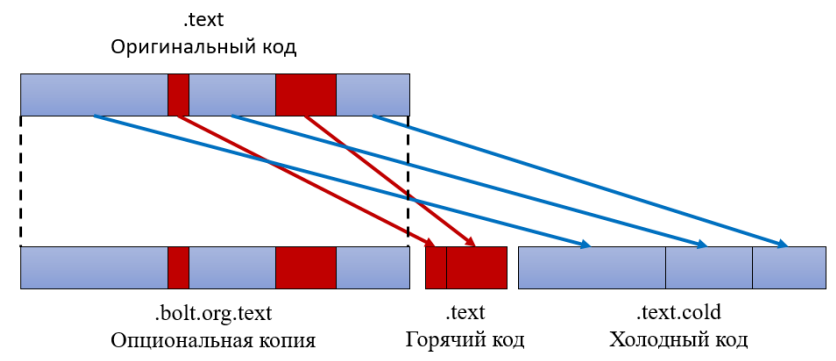
\includegraphics[width=0.7\textwidth]{pics/BoltAlgorithmOverview.png}
        \caption{Схема работы бинарного оптимизатора BOLT \cite{lisitsyn-disser}.}
        \label{fig:boltoverview}
    \end{figure}


    \section{Релокационная информация}
    Релокации - механизм, применяемый линкерами для связывания символов в программе с их конечными адресами в бинарном файле \cite{linker-overview}. Описание формата релокаций и их смысл являются частью спецификации формата исполняемого файла. Для ELF файлов, используемых в операционной системе Andrioid, статическая релокационная информация помещается в отдельные секции, имена которых помечены префиксами .rel или .rela. Эти секции содержат записи следующего формата \cite{aarch64-elf-docs}:
    \inputminted{c}{src/relocations.c}

    \begin{itemize}
        \item Поле r\_offset обычно кодирует адрес в памяти, к которому надо применить релокацию.
        \item Поле r\_info кодирует тип релокации и символ с которым релокация связана.
        \item Поле r\_addend есть только у релокаций типа rela и кодирует отступ от символа.
    \end{itemize}

    Статическая процедура связывания подразумевает вычисление адреса по релокационной информации и запись полученного значения по адресу, закодированному в поле r\_offset. Правила вычисления адреса отличаются в зависимости от типа релокации. Например, для релокаций типа \verb|R_AARCH64_PREL32|, означающих 32-битное смещение относительно PC (Program Counter), правило вычисления следующее:
    \begin{equation}
        V = S + A - P \mod 2^{32}
        \label{eq:RelocValue}
    \end{equation}
    Здесь $V$ - значение релокации, $S$ - адрес символа, $A$ - значение поля r\_addend, $P$ - значение поля r\_offset.


    \section{Таблицы переходов в архитектуре AArch64}
    \textit{Замечание:} В данной работе рассматриваются приложения скомпилированные для архитектуры AArch64 в режиме PIE. Поэтому все рассматриваемые конструкции в бинарном коде не должны зависеть от абсолютных адресов \cite{repica}.

    Таблица переходов в исполняемом PIE файле состоит из двух частей – шаблона доступа и массива смещений. Ее структура приведена на рисунке \ref{fig:jtoverview}.

    \begin{figure}[h!]
        \centering
        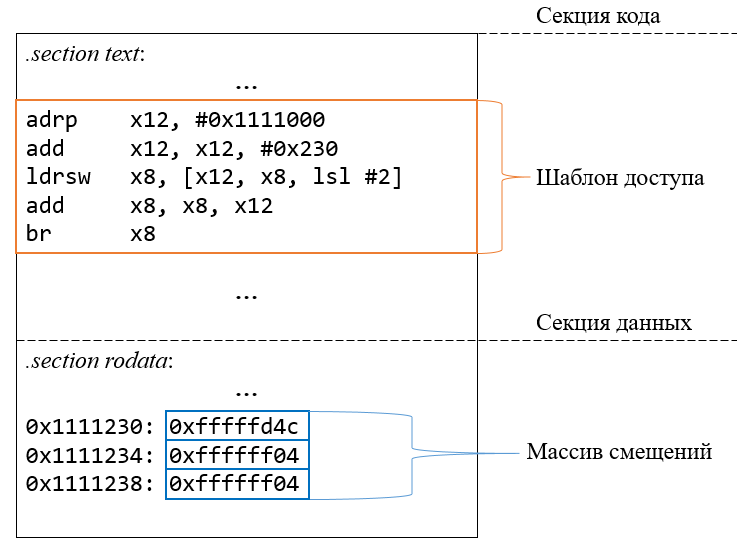
\includegraphics[width=0.7\textwidth]{pics/JumpTableOverview.png}
        \caption{Структура таблицы переходов в архитектуре ARM.}
        \label{fig:jtoverview}
    \end{figure}

    Шаблон доступа - это последовательность инструкций в программе, которая отвечает за формирование адреса и осуществление косвенного перехода по нему. Для формирования адреса используется массив смещений – участок памяти в секции данных, содержащий массив констант одинакового размера. Размер констант может варьироваться от 1 до 4 байт. Из логики работы инструкций шаблона доступа следует формула для подсчета адреса косвенного перехода:

    \begin{equation}
        TargetAddress = Base + sign\_extend_{64}(OffsetArray[Index]) \ll Shift
        \label{eq:jt_adr_calculation}
    \end{equation}

    В формуле \formref{eq:jt_adr_calculation} использованы следующие обозначения:

    \begin{itemize}
        \item $Target Address$ - адрес перехода.
        \item $Base$ - база отсчета адреса.
        \item $OffsetArray[Index]$ - элемент массива смещений с индексом $Index$.
        \item $sign\_extend_{64}$ - операция знакового расширения числа до 64 бит.
        \item $Shift$ - значение опционального битового сдвига влево. Может быть равно 0.
    \end{itemize}

    Такой алгоритм подсчета адреса позволяет выполнять в данной точке программы переход на разные адреса в зависимости от значения $Index$. При этом для определения адреса массива смещений используется зависящая от PC инструкция \verb|ADRP|. Сам массив содержит смещение адреса перехода относительно базы отсчета. Таким образом эта формула инвариантна относительно изменения адреса загрузки приложения в память, а значит может использоваться в PIE файлах.

    Примером высокоуровневой конструкции, которая компилируется в таблицу переходов, является \verb|switch-case| оператор из языков C и C++.

    Компилятор для целевой платформы генерирует всего два типа таблиц переходов. Они приведены в таблице \picref{tab:access_patterns_examples}. Типы отличаются способом формирования базы отсчета $Base$ и наличием релокаций для элементов массива смещений.

    \begin{table}[h!]
        \centering
        \begin{tabular}[h!]{|p{0.5\textwidth}|p{0.5\textwidth}|}
            \hline
            \inputminted[highlightlines={4}]{gas}{src/jump_table_BBend_type.s}
            &
            \inputminted{gas}{src/jump_table_Array_type.s}
            \\ \hline
            Шаблон доступа первого типа. В качестве $Base$ используется конец базового блока. Релокаций нет. &
            Шаблон доступа второго типа. В качестве $Base$ используется начало массива смещений. Есть релокации. \\
            \hline
        \end{tabular}
        \caption{Примеры шаблонов доступа.}
        \label{tab:access_patterns_examples}
    \end{table}

    \section{Таблица перехода с адресацией относительно кода}

    В случае шаблона доступа первого типа адресация происходит относительно кода. Инструкция \verb|adr| загружает в регистр адрес следующий за инструкцией косвенного перехода. Затем этот адрес используется в качестве базы адресации таблицы переходов. Таким образом формула вычисления адреса косвенного перехода становится:

    $$Target Address = (BranchAddress + 4) + sign\_extend_{64}(OffsetArray[Index]) \ll Shift$$

    где $BranchAddress$ - адрес инструкции косвенного перехода.

    В таблицах такого типа база отсчета и точки программы, на которые может передать управление таблица переходов, находятся в пределах одной исполняемой секции. Поэтому относительное смещение между ними не может измениться в результате процедуры связывания. По этой причине для элементов массива релокации не нужны.

    \section{Таблица перехода с адресацией относительно данных}

    В случае шаблона доступа второго типа адресация происходит относительно данных. За базу отсчета принимается начало массива смещений. Формула для расчета адреса перехода принимает следующий вид:
    $$TargetAddress = OffsetArray + sign\_extend_{64}(OffsetArray[Index])$$
    где $OffsetArray$ - адрес массива смещений.

    В таблицах такого типа база отсчета и точки программы, на которые может передать управление шаблон доступа, находятся в разных секциях. Из-за этого компилятор не может вычислить значения элементов в массиве смещений до процедуры связывания. Поэтому для записей в массиве смещений требуется релокационная информация. Она кодируется с помощью релокаций типа \verb|R_AARCH64_PREL32| \picref{fig:rodata_reloc}.

    \begin{figure}[h!]
        \centering
        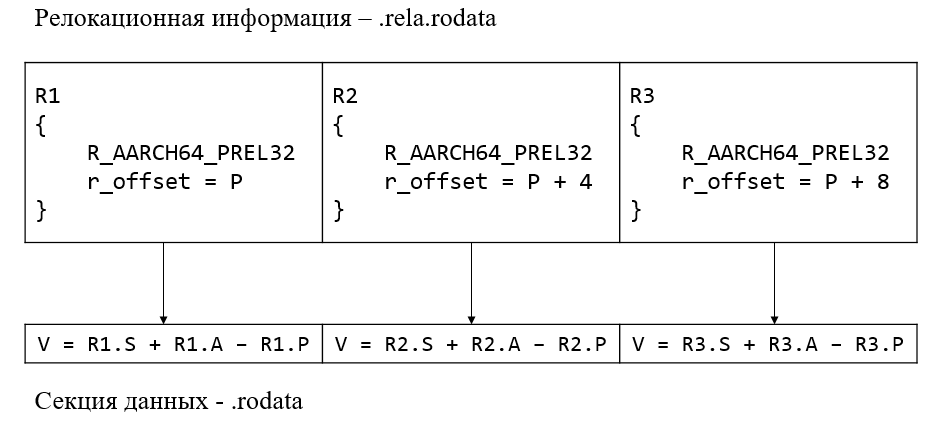
\includegraphics[width=0.8\textwidth]{pics/Relocations.png}
        \caption{Релокационная информация для массива смещений.}
        \label{fig:rodata_reloc}
    \end{figure}


    \section{Поддержка таблиц переходов в LLVM BOLT для AArch64}
    Существующий алгоритм обработки таблиц переходов LLVM BOLT детектирует только таблицы переходов с адресацией относительно кода. Оптимизатор запрещает изменение компоновки базовых блоков функций, в которых обнаружена такая таблица. Данное ограничение не позволяет получить прирост за счет локализации горячих блоков функции, но исключает возможность ошибок в таблице переходов, за счет PIE свойств кода.

    Второй тип таблиц переходов LLVM BOLT не детектирует. Вместо этого он полагается на анализ релокационной информации. Все релокации типа \verb|R_AARCH64_PREL32| обрабатываются единообразно, в том числе те что не относятся к таблицам переходов. BOLT пересчитывает значение релокаций на основе расположения объектов в памяти оптимизированного приложения:
    \begin{enumerate}
        \item Подсчитывается адрес на который указывает релокация в оригинальном адресном пространстве.
        \item Этот адрес отображается в адресное пространство оптимизированного приложения.
        \item Вычисляется значение релокации в новом адресном пространстве.
        \item Значение релокации записывается по адресу, закодированному в поле \verb|r_offset| релокации.
    \end{enumerate}
    Как будет показано далее, в случае таблиц переходов такой подход не работает - записи в массиве смещений оказываются невалидными.

    \chapter{Исследование и построение решения задачи}

    \section{Влияние оптимизаций на корректность таблиц переходов}
    % пересчет формулы
    % влияние на таблицы первого типа
    % влияние на таблицы второго типа
    % неявная зависимость, порождает ошибки в релокациях
    % Почему недостаточно просто setSimple

    Целевыми блоками таблицы переходов будем называть все базовые блоки, на которые может передать управление данная таблица переходов.

    В результате применения LLVM BOLT целевые блоки таблицы переходов могут изменить свой адрес. В таком случае оптимизатор должен исправить массив смещений. Пусть адрес целевого блока таблицы переходов $Target$ и база отсчета $Base$ после оптимизации стали равны $Target'$ и $Base'$ соответственно. Тогда согласно формуле \formref{eq:jt_adr_calculation}

    \begin{equation}
        Target' = Base' + sign\_extend_{64}(OffsetArray[Index]) \ll Shift
        \label{eq:target'}
    \end{equation}

    Для того чтобы данное равенство выполнялось в новом адресном пространстве, оптимизатору нужно изменить элемент массива смещений с индексом $Index$. Новое значение элемента массива можно выразить из равенства \formref{eq:target'}:

    \begin{equation}
        OffsetArray[Index]' = (Target' - Base') \gg Shift \mod 2^{8 \cdot sizeof(OffsetArray[Index])}
        \label{eq:offset'}
    \end{equation}

    В последнем равенстве нужно учесть, что адреса $Target'$ и $Base'$ занимают в 64-битной архитектуре 8 байт, а элемент массива может занимать 1, 2 или 4 байта. Поэтому результат вычислений в правой части должен быть обрезан до размера элемента массива.

    Формула \formref{eq:offset'} показывает, что значение элемента массива смещений зависит только от разности $Target'$ и $Base'$, но не от их абсолютных значений. Таким образом такая таблица переходов может быть использована в PIE исполняемых файлах.

    \subsection{Влияние оптимизаций на таблицы перехода с адресацией относительно кода}

    В случае детекции таблиц переходов с адресацией относительно кода LLVM BOLT запрещает изменение относительного расположения базовых блоков в данной функции - функция может перемещаться только целиком. Таким образом выполняются равенства:
    \begin{align*}
        Target - Base &= Target' - Base'\\
        \Rightarrow OffsetArray[Index] &= OffsetArray[Index]'
    \end{align*}
    элементы массива оказываются валидными в новом адресном пространстве без дополнительной модификации со стороны оптимизатора. Данная стратегия не работает, если целевой блок таблицы переходов окажется в другой функции, но такие случаи LLVM BOLT не обрабатываются.

    \subsection{Влияние оптимизаций на таблицы перехода с адресацией относительно данных}

    Рассмотрим таблицы перехода с адресацией относительно данных. Так как LLVM BOLT их не детектирует, то смещение между адресами целевых блоков и базой отсчета в новом адресном пространстве может измениться.
    \begin{align*}
        Target - Base &\neq Target' - Base'\\
        \Rightarrow OffsetArray[Index] &\neq OffsetArray[Index]'
    \end{align*}
    Требуется изменить записи в массиве в соответствии с формулой \formref{eq:offset'}. Для модификации массива оптимизатор полагается на механизм релокаций.

    \begin{listing}[h!]
        \inputminted{gas}{src/jump_table_Array_pseudo.s}
        \caption{Псевдокод шаблона доступа с адресацией относительно данных.}
        \label{fig:jt_datarel_pseudo}
    \end{listing}

    На каждый элемент массива смещений в исполняемом файле есть релокация типа \verb|R_AARCH64_PREL32|. Поле \verb|r_offset| в этих релокациях равно адресам элементов массива. Тогда согласно шаблону доступа (\coderef{fig:jt_datarel_pseudo}) значение релокации $V$ в оригинальном адресном пространстве должно удовлетворять выражению:
    \begin{align}
        Target &= OffsetArray + sign\_extend_{64}(V)
        \label{eq:datarel_target_val}\\
        V &= Target - OffsetArray \mod 2^{32}
        \label{eq:datarel_reloc_val_target}
    \end{align}
    С другой стороны по правилу вычисления значения релокации \formref{eq:RelocValue}
    \begin{equation}
        V = S + A - P \mod 2^{32}
        \label{eq:datarel_reloc_val}
    \end{equation}
    В данном случае $P$ равно значению поля \verb|r_offset|, то есть адресу элемента массива. Адрес элемента массива получается прибавлением $Index$ к базе отсчета $OffsetArray$. Тогда выражение \formref{eq:datarel_reloc_val} принимает вид.
    \begin{equation*}
        V = S + A - OffsetArray - 4 \cdot Index \mod 2^{32}
    \end{equation*}
    Подставим сюда выражение \formref{eq:datarel_reloc_val_target} и выразим закодированный в релокации адрес $S + A$.
    \begin{equation}
        S + A = Target + 4 \cdot Index \mod 2^{32}
        \label{eq:true_reloc_val}
    \end{equation}
    Таким образом, из логики работы инструкций в шаблоне доступа и правила вычисления значений релокаций следует, что в исходном исполняемом файле релокации элементов массива смещений не указывают на адрес целевого базового блока. Вместо этого в них закодирован адрес целевого блока смещенный на $4 \cdot Index$. Это порождает неявную зависимость значений всех элементов массива смещений от адреса начала массива.

    Для формирования релокационной информации оптимизированного приложения LLVM BOLT отображает адрес закодированный в оригинальных релокациях в новое адресное пространство. Оригинальный адрес вычисляется по правилу общему для всех релокаций \verb|R_AARCH64_PREL32|.
    $$S + A = V + P$$
    Согласно \formref{eq:true_reloc_val} этот адрес не соответствует адресу целевого базового блока, поэтому адрес, который получает LLVM BOLT в адресном пространстве оптимизированного приложения, в общем случае является невалидным и при формировании новых релокаций в оптимизированном файле порождает невалидные записи в массиве.

    Пример ситуации, которая приводит к возникновению ошибок представлен на \picref{fig:bugcase}. Значение смещения от адреса базового блока $4 \cdot Index$ может оказаться больше чем размер самого базового блока и попасть в следующий базовый блок. В таком случае если в оптимизированном приложении разность адресов между этими двумя блоками изменится на $\Delta$, то итоговое значение релокации изменится на $\Delta$. Это приведет к тому, что адрес перехода, получаемый из связанного с релокацией элемента массива, также изменится на $\Delta$ и станет не равен адресу целевого блока в оптимизированном адресном пространстве. Таким образом при оптимизации нарушается целостность потока управления.

    \begin{figure}[h!]
        \centering
        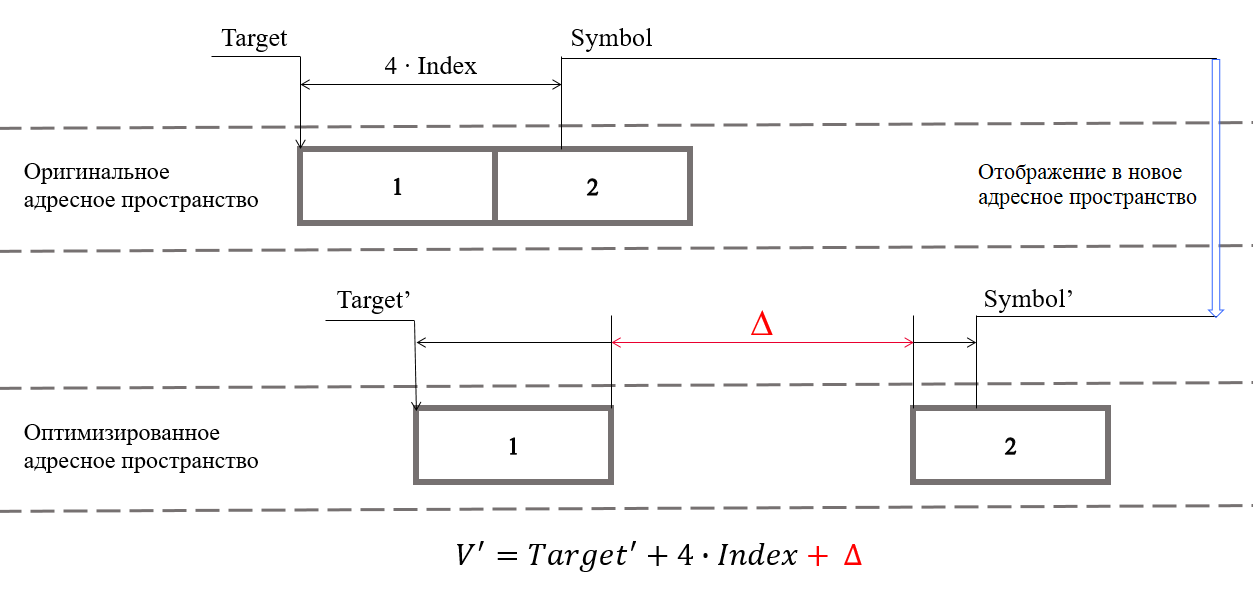
\includegraphics[width=0.8\textwidth]{pics/bugcase.png}
        \caption{Пример ошибки при пересчете значения релокации.}
        \label{fig:bugcase}
    \end{figure}

    Для корректной обработки таблиц переходов при пересчете релокаций следует опираться не на значение релокации, а непосредственно на адрес целевого блока. Получить адрес целевого блока $Target$ можно зная значение релокации и адрес начала массива смещений по формуле \formref{eq:datarel_target_val}. Полученный адрес следует отобразить в адресное пространство оптимизированного приложения. Затем сформировать новую релокацию:
    \begin{align*}
        P' &= P\\
        S' &= Target'\\
        A' &= P - OffsetArray
    \end{align*}
    Значение такой релокации удовлетворяет выражению \formref{eq:datarel_reloc_val_target} в адресном пространстве оптимизированного приложения.
    $$V' = S' + A' - P' = Target' - OffsetArray \mod 2^{32}$$
    Подобным образом нужно пересчитать только те релокации, которые относятся к массиву смещений данной таблицы переходов. То есть для произвольно взятой релокации секции данных нужно иметь возможность определить, принадлежит ли она массиву смещений. Так как элементы массива должны идти подряд, начиная с адреса начала массива, задача определения принадлежности каждого следующего элемента массиву сводится к определению его размера.

    Таким образом для правильной обработки таблицы переходов с адресацией относительно данных требуется вычислить адрес массива смещений этой таблицы, или, что тоже самое, определить базу отсчета, и определить размер массива смещений. В существующем алгоритме LLVM BOLT ошибки связаны с тем, что каждый элемент массива смещений трактуется как начало массива.

    \section{Статический анализ таблиц переходов с адресацией относительно данных}
    % вычисление начала массива по инструкциям
    % проблема определения размера массива
    % система уравнений с релокациями
    Задача анализа таблиц переходов в бинарном файле оригинального приложения состоит в определении границ массива смещений. Обладая этой информацией, можно статически определить адреса всех целевых блоков таблицы. Зная адреса целевых блоков, можно корректно сформировать массив смещений для оптимизированного файла.

    \subsection{Определение начала массива смещения}
    Начало массива смещений определяется по шаблону доступа таблицы переходов. Инструкции \verb|adrp| и \verb|add| в шаблоне отвечают за формирование адреса массива смещений. \verb|adrp| загружает в регистр старшие биты с 12 по 31, инструкция \verb|add| добавляет к адресу младшие 12 бит (с 0 по 11). Таким образом, по аргументам этой пары инструкций можно установить адрес начала массива смещений. Задача сводится к нахождению в массиве инструкций исходного приложения шаблона доступа. В общем случае, инструкции шаблона доступа могут идти не подряд. Поэтому поиск шаблона осуществляется с помощью анализа графа потока данных по следующему алгоритму (обозначения, используемые в алгоритме, отображены в \coderef{fig:template_search_algo}):

    \begin{enumerate}
        \item В массиве инструкций исходного приложения найти инструкцию косвенного перехода \verb|br reg1|.
        \item Найти инструкцию сложения формата \verb|add reg1, reg2, reg3|, определяющую значение регистра \verb|reg1|.
        \item Найти инструкцию загрузки значения из памяти, использующую один из двух регистров \verb|reg2| или \verb|reg3| в качестве базы адресации. Пусть это будет \verb|reg3|.
        \item Найти инструкцию сложения \verb|add reg3, reg4, imm1| которая определяет значение базы адресации инструкции загрузки из памяти.
        \item Найти инструкцию \verb|adrp|, записывающую значение \verb|imm2| в регистр reg4.
        \item Если все инструкции были найдены, то они образуют шаблон доступа таблицы переходов. Адрес начала массива смещений равен сумме \verb|imm1| и \verb|imm2|.
    \end{enumerate}

    Пусть инструкция $i$ использует множество регистров $R$ как аргументы. Обозначим $Def(i)$ множество инструкций, которые при каком-либо сценарии исполнения программы могут определять значения регистров $R$ в данной точке. Алгоритм \ref{alg:template_lookup} определяет адрес массива смещений по шаблону доступа таблицы переходов.

    \begin{algorithm}[h!]
        \begin{algorithmic}
            \State $I$ - массив инструкций программы
            \State $JT$ - множество адресов таблиц переходов.
            \For {each $i \in I$ }
                \If {$i$ инструкция косвенного перехода}
                    \State $JT.insert(\Call{GetOffsetArrayStart}{$i$})$
                \EndIf
            \EndFor
            \Function{GetOffsetArrayStart}{$i_{br}$}
                \For {each $d \in Def(i_{br})$}
                    \If {$d$ инструкция сложения двух регистров}
                        \State $i_{load} \gets$ \Call{LoadLookup}{$d$}
                        \State $b_{add} \gets$ \Call{AddLookup}{$i_{load}$}
                        \State $b_{adrp} \gets$ \Call{AdrpLookup}{$b_{add}$}
                        \State $page \gets$ константный аргумент $b_{adrp}$
                        \State $offset \gets$ константный аргумент $b_{add}$
                        \State \Return $page + offset$
                    \EndIf
                \EndFor
            \EndFunction

            \Function{LoadLookup}{$i_{add}$}
            \For {each $d \in Def(i_{add})$}
                \If {$d$ инструкция загрузки из памяти по регистру}
                        \State \Return $d$
                    \EndIf
                \EndFor
            \EndFunction

            \Function{AddLookup}{$i_{load}$}
            \For {each $d \in Def(i_{load})$}
                \If {$d$ инструкция сложения регистра с числом}
                        \State \Return $d$
                    \EndIf
                \EndFor
            \EndFunction

            \Function{AdrpLookup}{$b_{add}$}
            \For {each $d \in Def(b_{add})$}
                \If {$d$ инструкция verb|adrp|}
                        \State \Return $d$
                    \EndIf
                \EndFor
            \EndFunction

        \end{algorithmic}
    \caption{Алгоритм поиска шаблона доступа таблицы переходов. Адреса массивов смещений всех таблиц перехода в программе записываются в $JT$.}
    \label{alg:template_lookup}
    \end{algorithm}

    \begin{listing}[h!]
        \inputminted{gas}{src/template_algo.s}
        \caption{Пояснения к алгоритму поиска шаблона доступа.}
        \label{fig:template_search_algo}
    \end{listing}

    \begin{figure}[h!]
        \centering
        \begin{tikzpicture} [node distance={15mm}, main/.style = {draw, ellipse}]
            \node[main] (1) { \verb|adrp reg4, imm2|};
            \node[main] (2) [below of=1] { \verb|add reg3, reg4, imm1|};
            \node[main] (3) [below of=2] { \verb|ldrsw reg2, [reg3, reg, lsl #2]|};
            \node[main] (4) [below of=3] { \verb|add reg1, reg3, reg2|};
            \node[main] (5) [below of=4] { \verb|br reg1|};
            \draw[->] (1) -- (2) node [midway, right] {\verb|reg4|};
            \draw[->] (2) -- (3) node [midway, right] {\verb|reg3|};
            \draw[->] (2) to [out=0,in=0,looseness=2.5] node [midway, right] {reg3} (4) ;
            \draw[->] (3) -- (4) node [midway, right] {\verb|reg2|};
            \draw[->] (4) -- (5) node [midway, right] {\verb|reg1|};
        \end{tikzpicture}
        \caption{Граф потока данных для примера \coderef{fig:template_search_algo}.}
    \end{figure}

    \section{Уравнения потока данных}
    Для поиска шаблона доступа используется граф потока данных. Построение такого графа подразумевает решение definition-use задачи для машинных инструкций. В данной работе для этого был использован метод уравнений потока данных для задачи доступных определений (Reaching definitions).

    При обработке бинарного файла LLVM BOLT конструирует граф потока управления. Вершинами данного графа являются базовые блоки. Каждый блок содержит последовательность линейно исполняемых инструкций, заканчивающихся инструкцией перехода. Этот граф используется для построения и решения уравнений потока данных.

    Определение регистра - выражение, меняющее значение регистра, например, инструкция загрузки значения из памяти в данный регистр. Определение регистра $r$ доступно в точке программы $P$, если в графе потока управления существует путь от определения $r$ до точки $P$, на котором значение $r$ не изменяется. Если на пути встречается другое определение $r$, то говорят что оно "убивает" первое определение. Задача доступных определений состоит в нахождении всех определений регистра $r$ доступных в данной точке программы $P$.

    Требуется вычислить доступные определения в точках до и после каждой инструкции в программе. Для этого в каждой точке формулируются соотношения, которые оперируют четырьмя логическими величинами:

    \begin{itemize}
        \item[\textbf{in}] Определение достигает точки перед исполнением инструкции.
        \item[\textbf{out}] Определение достигает точки после исполнения инструкции.
        \item[\textbf{gen}] Инструкция создает новое определение.
        \item[\textbf{kill}] Инструкция убивает определение.
    \end{itemize}

    В каждом случае \textit{gen} и \textit{kill} это величины которые мы можем легко определить для каждой инструкции, основываясь на логике ее работы, а \textit{in} и \textit{out} это величины, которые мы хотим в конечном счете установить. Все эти величины являются логическими функциями от инструкции $i$. Для величин \textit{gen} и \textit{kill} должно выполняться условие:

    $$\textit{gen(i)} \wedge \textit{kill(i)} = \text{FALSE}$$

    Теперь можно определить несколько типов уравнений с введенными величинами на графе потока управления программы.\\
    \textbf{Граничные условия} Определяют значения логических величин на входе или выходе из программы.\\
    \textbf{Уравнения распространения} Определяют как значения распространяются из одного базового блока в другой.\\
    \textbf{Уравнения переноса} Определяет как значения изменяются одной инструкцией.

    Есть два основных типа задач на поток данных: те в которых значения распространяются в направлении исполнения программы (прямые задачи), и те в которых значения распространяются в направлении противоположном исполнению программы (обратные задачи). Величины \textit{in}, \textit{out} и прочие представляются как битовые вектора, в которых каждое измерение соответствует какому-то определению в программе.

    Задача доступных определений относится к прямым задачам. Обозначим $s$ точку входа в программу (первая инструкция в графе потока управления), $\text{pred}(i)$ - все инструкции, имеющие ребро в инструкцию $i$ в графе потока управления (поток управления - направленный граф). Тогда уравнения для задачи доступных определений:
    \begin{align*}
        in(s) &= \emptyset \\
        in(i) = \bigcap_{x \in \text{pred}(i)}&out(x) \text{ for } i \neq s\\
        out(i) = (in(i) - &kill(i)) \cup gen(i)
    \end{align*}

    Чтобы построить граф потока данных, значения битовых векторов вычисляются по приведенным выше правилам для каждой инструкции в графе потока управления. Из-за наличия циклов в графе, недостаточно обойти весь граф один раз. Поэтому алгоритм применяется рекурсивно. Изначально в очередь обработки попадают все инструкции из графа. Далее они извлекаются по одной. Для извлеченной инструкции вычисляется значение \textit{out} множества. Если значение этого множества изменилось, то в очередь помещаются все инструкции, которые идут в графе потока управления после данной. Таким образом алгоритм продолжается до тех пор, пока в графе потока данных происходят изменения.

    % TODO: Тоже можно псевдокод при желании. И замечания по поводу сходимости графов

    В результате применения данного алгоритма для каждой инструкции можно сказать, какая инструкция определяет регистры, используемые данной инструкцией. Эта информация необходима для описанного выше алгоритма поиска шаблона доступа.

    \section{Вычисление размера таблицы переходов}
    % Проверка принадлежности релокации по уравнениям
    % Эвристика конкатенации релокаций
    % Расширенный шаблон доступа
    % Алгоритм анализа расширенного
    % Незадетектированные случаи
    Целевые адреса связаны со значением релокаций следующим равенством:
    $$Target = Base + V$$
    Это выражение выполняется только для релокаций, которые относятся к массиву смещений с адресом начала $Base$. По этой причине, чтобы правильно определить все множество целевых блоков таблицы переходов, нужно знать размер массива.

    \subsection{Оценка размера массива смещений по релокационной информации} \label{sec:reloc_estimate}

    Элементы массива располагаются в памяти последовательно. Для каждого элемента существует релокация с полем \verb|r_offset| равным адресу этого элемента. Основываясь на этих фактах, можно предложить способ оценки размера массива по релокационной информации. Он состоит в подсчете количества релокаций, которые начинаются с адреса $Base$ и идут подряд. Псевдокод этого метода приведен в алгоритме \ref{alg:reloc_cat_estimate}.

    \begin{algorithm}
    \begin{algorithmic}
        \State $Len \gets 0$
        \State $Addr \gets Base$
        \While{Relocation at $Addr$ is R\_AARCH64\_PREL32}
            \State $Len \gets Len + 1$
            \State $Addr \gets Addr + 4$
        \EndWhile
    \end{algorithmic}
    \caption{Алгоритм оценки размера массива смещений по релокациям. Вычисляет количество элементов массива в переменной $Len$.}
    \label{alg:reloc_cat_estimate}
    \end{algorithm}

    \begin{figure}[h!]
        \centering
        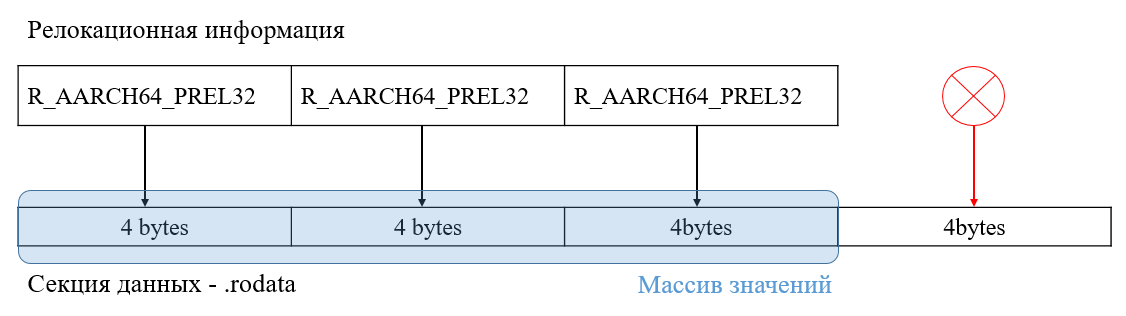
\includegraphics[width=\textwidth]{pics/reloc_cat_estimate.png}
        \caption{К алгоритму вычисления размера массива по релокациям.}
        \label{fig:reloc_cat_estimate}
    \end{figure}

    Этот алгоритм имеет большой недостаток. Если после массива смещений окажутся релокации типа \verb|R_AARCH64_PREL32|, не относящиеся к таблице переходов, то посчитанный размер окажется больше реального значения.

    \subsection{Оценка размера массива смещений по расширенному шаблону доступа} \label{sec:template_estimate}

    Второй предлагаемый метод оценки размера массива основывается на анализе инструкций в коде программы, также как и метод поиска шаблона доступа. Рассмотрим расширенный шаблон доступа таблицы переходов. Он приведен в \coderef{fig:ext-acc-template}. По сравнению с обычным шаблоном, рассмотренным ранее, здесь добавлены еще две инструкции - инструкция сравнения \verb|cmp| и инструкция условного перехода \verb|b.hi|. С точки зрения логики программы эти инструкции отвечают за проверку того, что значение $Index$ лежит в пределах размера массива. Схематично граф потока управления изображен на рисунке \picref{fig:ext-template-cfg}. Регистр, используемый как индекс в массиве смещений, сравнивается с константой равной размеру массива минус 1. В случае, если индекс оказывается больше константы, то инструкции шаблона доступа не исполняются. Такую логику работы имеет, например, ключевое слово \verb|default| из языков C и C++.

    \begin{listing}[h!]
        \inputminted{gas}{src/ext_template.s}
        \caption{Пример расширенного шаблона доступа.}
        \label{fig:ext-acc-template}
    \end{listing}

    \begin{figure}[h!]
        \centering
        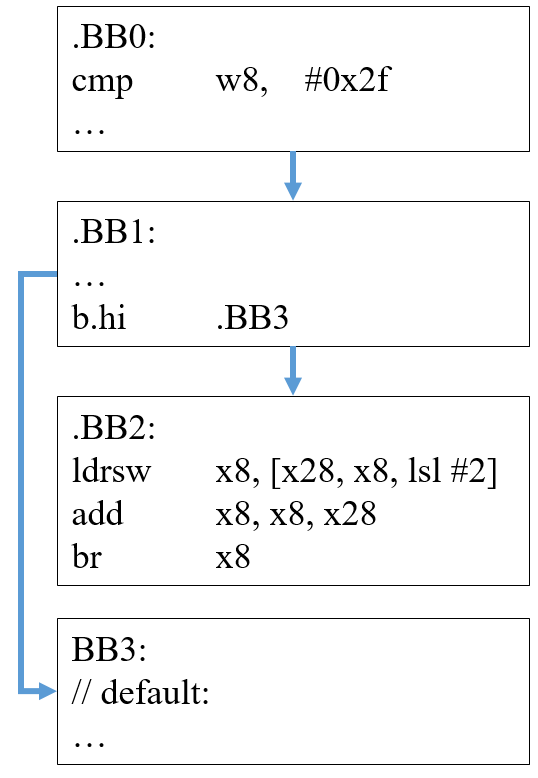
\includegraphics[width=0.4\textwidth]{pics/ext-template-cfg.png}
        \caption{Граф потока управления для расширенного шаблона доступа таблицы переходов.}
        \label{fig:ext-template-cfg}
    \end{figure}

    Для определения размера массива смещений по расширенному шаблону доступа достаточно по графу потока данных найти инструкцию сравнения \verb|cmp|. Определение флагов сравнения, порождаемое этой инструкцией, должно быть доступно инструкции условного перехода \verb|b.hi| в смысле определения, данного выше для задачи доступных определений. Константный аргумент инструкции \verb|cmp| позволяет определить размер массива смещений. Данный подход никак не опирается на релокационную информацию и использует только анализ исполняемого кода приложения. Обозначим $BB_{load}$ базовый блок, содержащий обращение к массиву смещений (инструкцию загрузки из памяти), $pred(BB)$ - множество базовых блоков, имеющих ребро ведущее к блоку $BB$ в графе потока управления. При обработке графа нужно учитывать, что искомый блок с инструкцией \verb|cmp| может не быть непосредственным предшественником блока $BB_{load}$. Псевдокод приведен в алгоритме \ref{alg:cmp_estimate}.

    \begin{algorithm}[h]
    \begin{algorithmic}
        \State $Q \gets \text{пустая очередь}$
        \State $Visited \gets \text{пустая очередь}$
        \State $Len \gets 0$
        \State $Q.push(pred(BB_{load}))$
        \While {$Q$ not empty}
            \State $BB \gets Q.pop()$
            \If {$Visited$ содержит $BB$}
                \State пропустить итерацию цикла % Я могу написать здесь continue?
            \EndIf
            \State $Visited.push(BB)$
            \If {$BB$ содержит инструкцию b.hi}
                \For {each определения доступные b.hi}
                    \If {определение - инструкция cmp}
                        \State $Imm$ - аргумент cmp
                        \State $Len \gets Imm + 1$
                        \State \Return
                    \EndIf
                \EndFor
            \Else
                \For {each $p \in pred(BB)$}
                    \If {$Visited$ не содержит $p$}
                        \State $Q.push(p)$
                    \EndIf
                \EndFor
            \EndIf
        \EndWhile
    \end{algorithmic}
    \caption{Алгоритм оценки размера массива смещений по расширенному шаблону доступа. Количество элементов в массиве смещений записывается в переменную $Len$.}
    \label{alg:cmp_estimate}
    \end{algorithm}

    Алгоритм анализа расширенного шаблона доступа позволяет точно определить размер массива смещений.

    \section{Устойчивость алгоритма анализа к изменению шаблона доступа} \label{sec:stability-analysis}
    Алгоритм анализа таблиц переходов полагается на поиск определенных последовательностей инструкций в коде приложения. В общем случае, искомые инструкции могут располагаться в бинарном коде приложения произвольным образом. Однако алгоритм работает с представлением программы в форме графа потока управления и графа потока данных. Поэтому он не зависит от расположения инструкций в бинарном файле приложения.

    В некоторых случаях компилятор может генерировать последовательности инструкций, которые реализуют ту же самую логику, но отличаются набором инструкций от заданного шаблона. Примеры таких последовательностей приведены в \coderef{fig:single_nop} и \coderef{fig:single_mov}.

    \begin{listing}[h!]
        \inputminted[highlightlines={3}]{gas}{src/single_mov.s}
        \caption{Пример шаблона доступа с инструкцией mov.}
        \label{fig:single_mov}
    \end{listing}

    \begin{listing}[h!]
        \inputminted[highlightlines={3}]{gas}{src/single_nop.s}
        \caption{Пример шаблона доступа с инструкцией nop.}
        \label{fig:single_nop}
    \end{listing}

    Количество сохраняющих логику преобразований шаблона доступа бесконечно велико. Например, шаблон можно бесконечно дополнять инструкциями \verb|nop| не выполняющими никакого действия (пример \coderef{fig:many_nops}). Однако такое преобразование не влияет на граф потока данных, поэтому не влияет и на алгоритм анализа шаблона доступа.

    Существуют более сложные случаи преобразований, меняющие граф потока данных, но сохраняющие логику работы шаблона доступа таблицы переходов (пример \coderef{fig:single_mov}). Назовем две последовательности инструкций в потоке исполнения программы равными с учетом множества регистров $R$, если их исполнение приводит программу в одну и ту же точку графа потока управления, и в этой точке значения всех регистров множества $R$ равны для обеих последовательностей. Рассмотрим пример шаблона доступа \coderef{fig:single_mov} и покажем, что существует бесконечное множество последовательностей равных шаблону доступа с учетом регистров $\{reg3,\ reg4,\ reg5,\ reg6\}$. Действительно, шаблон можно дополнить произвольным количеством пар инструкций \verb|mov| копирования значений из одного регистра в другой (\coderef{fig:many_movs}). Каждая новая пара инструкций \verb|mov| меняет граф потока данных, но оставляет последовательности равными с учетом регистров $\{reg3,\ reg4,\ reg5,\ reg6\}$.

    \begin{listing}[h!]
        \inputminted[highlightlines={3-6}]{gas}{src/nops.s}
        \caption{Пример шаблона доступа с множеством инструкций nop. Граф потока данных не изменяется. Логика работы не изменяется.}
        \label{fig:many_nops}
    \end{listing}

    \begin{listing}[h!]
        \inputminted[highlightlines={3-8}]{gas}{src/movs.s}
        \caption{Пример шаблона доступа с множеством инструкций mov. Граф потока данных изменяется. Логика работы не изменяется.}
        \label{fig:many_movs}
    \end{listing}

    Хороший алгоритм поиска шаблона доступа должен быть устойчив к сохраняющим равенство преобразованиям шаблона, то есть уметь находить шаблон доступа в любых последовательностях инструкций, возможно отличающихся от шаблона доступа набором инструкций, но обладающих такой же логикой работы. Обработать все такие последовательности в общем случае невозможно по двум причинам:
    \begin{enumerate}
        \item Как было показано число таких последовательностей бесконечно велико. В общем случае граф потока данных, сохраняющий логику шаблона доступа таблицы переходов, может иметь произвольную сложность.
        \item Статический анализ приложения не позволяет обработать последовательности в которых значения регистров сначала сохраняются, а потом загружаются из памяти (\coderef{fig:memory-error}), или в которых присутствуют инструкции косвенного перехода.
    \end{enumerate}

    \begin{listing}[h!]
        \inputminted[highlightlines={3,5}]{gas}{src/error_example.s}
        \caption{Пример шаблона доступа с передачей значения через память. Такой случай нельзя обработать статически.}
        \label{fig:memory-error}
    \end{listing}

    Код реальных приложений, которые являются целевыми для LLVM BOLT, оптимизируется и генерируется компилятором в процессе создания программы. Поэтому можно предположить, что в абсолютном большинстве случаев бинарный код шаблона доступа будет минимален или близок к минимальному. Тогда обработка минимального шаблона и небольшого числа наиболее частых его модификаций должны обеспечить достаточную надежность в определении таблиц переходов.

    \chapter{Результаты и обсуждение}
    Описанные в рамках данной работы алгоритмы детекции и анализа таблиц переходов были реализованы в инфраструктуре бинарного оптимизатора LLVM BOLT. Встраивание результатов работы в существующую иерархию классов LLVM BOLT позволяет оптимизатору формировать корректные таблицы переходов в адресном пространстве оптимизированного приложения.

    \section{Сравнение алгоритмов оценки размера массива смещений} \label{sec:estimate-comparision}
    В работе предложено два алгоритма для оценки размера массива смещений.
    \begin{enumerate}
        \item Алгоритм оценки размера массива смещений по релокационной информации в главе \ref{sec:reloc_estimate}.
        \item Алгоритм оценки размера массива смещений по расширенному шаблону доступа в главе \ref{sec:template_estimate}.
    \end{enumerate}
    Первый алгоритм проще в смысле реализации, однако обладает рядом важных недостатков по сравнению со вторым. Для обоих алгоритмов существуют примеры входных данных, которые приведут к ошибке в оценке размера таблицы переходов. Однако в случае алгоритма анализа релокаций ошибка не детектируется, тогда как в случае алгоритма анализа расширенного шаблона доступа всегда точно известно если оценить размер не удалось. Это свойство делает второй алгоритм более подходящим для промышленных продуктовых решений, каким является бинарный оптимизатор LLVM BOLT.

    Второе преимущество анализа по шаблону доступа, состоит в том, что этот подход не использует дополнительную информацию, в частности, релокации. Это свойство полезно при оптимизации приложений для конечных пользователей. В целях уменьшения размера из бинарных файлов таких приложений часто удаляют релокации, например, с помощью инструмента \verb|strip| \cite{strip}. Анализ релокаций в таких бинарных файлах невозможен. Метод анализа по шаблону доступа позволяет обрабатывать бинарные файлы без релокационной информации.

    Преимущества метода анализа по расширенному шаблону обосновывают выбор этого алгоритма для использования в LLVM BOLT.

    \section{Оценка устойчивости алгоритма определения размера массива смещений к изменению шаблона доступа}
    Для проверки гипотезы о надежности определения таблиц переходов по минимальному шаблону, высказанной в главе \ref{sec:stability-analysis}, были подсчитаны метрики, характеризующие точность определения таблиц переходов. Для каждого приложения $a$ в тестовом наборе были посчитаны полное количество таблиц переходов $N_a$ и количество таблиц, для которых удалось установить адрес начала и конца массива смещений $N^{correct}_a$. По этим данным были посчитаны количество приложений, в которых все таблицы обработаны полностью верно $N^{correct}$, и суммарное количество приложений, в которых встретились таблицы перехода $N$. Далее были вычислены следующие метрики:
    \begin{itemize}
        \item Доля приложений без ошибок:
        $$A = \frac{N^{correct}}{N}$$
        \item Средняя доля неверно обработанных таблиц среди приложений с ошибками:
        $$E = \frac{\sum_a \frac{N_a - N^{correct}_a}{N_a}}{N - N^{correct}}$$
    \end{itemize}

    Полученные значения приведены в таблице \ref{tab:metrics}.

    \begin{table}[h!]
        \centering
        \begin{tabular}{|c|c|}
            \hline
            Метрика & Значение \% \\ \hline
            $A$ & $99.4\%$ \\ \hline
            $E$ &  $0.33\%$ \\ \hline
        \end{tabular}
        \caption{Метрики надежности алгоритма анализа таблиц переходов.}
        \label{tab:metrics}
    \end{table}

    Полный размер тестового набора составил 621 приложение. Из них 170 содержали таблицы переходов. Ошибка обработки была обнаружена лишь в 1 приложении. В нем для 2 таблиц из 606 не получилось вычислить размер массива смещений.

    Близкое к 100\% значение $A$, говорит о том, что абсолютное большинство приложений обрабатывается полностью корректно. Это означает что приложения с проблемными случаями встречаются очень редко. Близкое к 0\% значение $E$ говорит о том, что в тех приложениях, где ошибки все-таки встречаются, их очень мало.

    \section{Оценка улучшения стабильности работы оптимизатора} \label{sec:results}
    Для оценки результатов работы было проведено повторное исследование стабильности LLVM BOLT на том же наборе тестов, который выявил проблемы при оптимизации таблиц переходов. Ожидалось, что внесенные изменения повысят процент приложений, работающих корректно после оптимизации. Результаты тестирования показали, что все 602 теста из набора работают корректно после оптимизации. Таким образом, подход предложенный в данной работе решает проблему оптимизации приложений с таблицами переходов.

    \chapter{Заключение}
    В ходе работы была исследована корректность работы приложений после оптимизации с помощью LLVM BOLT для архитектуры AArch64. В открытой версии инструмента были выявлены ошибки формирования таблиц переходов в оптимизированных приложениях. В 24 из 602 (4\%) тестовых приложений после оптимизации наблюдались ошибки времени исполнения.

    Были предложены алгоритмы поиска, анализа и модификации таблиц переходов для генерации корректных оптимизированных приложений. Алгоритм поиска использует графы потока управления и потока данных приложения для обнаружения последовательностей инструкций, которые исполняют логику таблиц переходов.

    Алгоритм анализа определяет начало и размер массива смещений - области данных, содержащей информацию о целевых адресах таблицы переходов. Определение границ массива смещений позволяет статически вычислить все целевые базовые блоки таблицы. Для оценки размера массива смещений предложено два способа - с использованием релокационной информации (глава \ref{sec:reloc_estimate}) и по расширенному шаблону доступа (глава \ref{sec:template_estimate}). Приведено сравнение двух способов (глава \ref{sec:estimate-comparision}), обосновывающее выбор второго алгоритма для использования в LLVM BOLT.

    Описанные в работе алгоритмы реализованы как часть бинарного оптимизатора LLVM BOLT.

    Дана численная оценка частоты возникновения ошибок при определении размера массива смещений по шаблону доступа таблицы переходов. Полученные значения приведены в таблице \ref{tab:metrics}. Результаты показывают высокую надежность алгоритма.

    Исследована корректность работы приложений, оптимизированных с помощью LLVM BOLT с применением описанных в данной работе техник обработки таблиц переходов (глава \ref{sec:results}). Все 602 приложения из тестового набора работают корректно при использовании модифицированной версии оптимизатора. Таким образом, достижением данной работы является существенное улучшение стабильности работы LLVM BOLT для архитектуры AArch64.

    \backmatter

    \printbib

\end{document}